\documentclass[12pt]{article}
\usepackage[mathscr]{euscript}
\DeclareSymbolFont{rsfs}{U}{rsfs}{m}{n}
\DeclareSymbolFontAlphabet{\mathscrsfs}{rsfs}

%++++++++++++++++++++++++++++++++++++++++
% Don't modify this section unless you know what you're doing!
\documentclass[letterpaper,12pt]{article}
\usepackage{tabularx} % extra features for tabular environment
\usepackage{multirow} % multiple rows in the table
\usepackage{physics}  % improve math presentation
\usepackage{graphicx} % takes care of graphic including machinery
\usepackage[margin=1in,letterpaper]{geometry} % decreases margins
\usepackage{cite} % takes care of citations
\usepackage{float}
\usepackage[final]{hyperref} % adds hyper links inside the generated pdf file
\usepackage{url}
\usepackage{natbib}
\usepackage[labelfont=bf]{caption}
\hypersetup{
	colorlinks=true,       % false: boxed links; true: colored links
	linkcolor=blue,        % color of internal links
	citecolor=blue,        % color of links to bibliography
	filecolor=magenta,     % color of file links
	urlcolor=blue         
}
% ++++++++++++++++++++++++++++++++++++++++

\newcommand{\labfig}[4]{
  \begin{figure}[H]
    \centering
    \includegraphics[width=#1cm]{#2}
    \caption{#3}
    \label{#4}
  \end{figure}}


\begin{document}

\title{Title of the Report}
\author{A. Partner, B. Partner, and C. Partner}
\date{\today}
\maketitle

\begin{abstract}
In this experiment we studied a very important physical effect by measuring the
dependence of a quantity $V$ of the quantity $X$ for two different sample
temperatures.  Our experimental measurements confirmed the quadratic dependence
$V = kX^2$ predicted by Someone's first law. The value of the mystery parameter
$k = 15.4\pm 0.5$~s was extracted from the fit. This value is
not consistent with the theoretically predicted $k_{theory}=17.34$~s. We attribute this
discrepancy to low efficiency of our $V$-detector.
\end{abstract}


\section{Introduction/Objective}

The very important physical effect has applications to astronomy, nuclear physics, condensed matter, and more. 


\section{Theory/Background}

Here give a brief summary of the physical effect of interest and provide
necessary equations. Here is how you insert an equation. According to
references~\cite{melissinos, Cyr, Wiki} the dependence of interest is given

\section{Procedures}

Give a schematic of the experimental setup(s) used in the experiment (see
figure~\ref{fig:Fig1}). Give the description of  abbreviations
either in the figure caption or in the text. Write a description of what is
going on. 

Don't forget to list all important steps in your experimental procedure!

Use active voice either in past or present through all the report and be
consistent with it:
The laser light comes  from to ... and eventually arrived to the
balanced photodiode as seen in the figure~\ref{fig:Fig1}.

Sentences in the past voice while correct are generally considered hard to read
in large numbers. The laser light was directed to ..., wave plates were set
to ... etc.


\section{Data and Analysis}

In this section you will need to show your experimental results. Use tables and
graphs when it is possible. Table~\ref{tbl:bins} is an example.

\begin{table}[ht]
\begin{center}
\caption{Every table needs a caption.}
\label{tbl:bins} % spaces are big no-no withing labels
\begin{tabular}{|cc|} 
\hline
\multicolumn{1}{|c}{$x$ (m)} &
\multicolumn{1}{c|}{$V$ (V)} \\
\multicolumn{1}{c|}{$V$ (V)} \\
\multirow{2}{*}{Multirow}&X\\
\multirow{2}{*}{Multirow}&Y\\
\multirow{2}{*}{Multirow}&Z\\
\hline
0.0044151 &   0.0030871 \\
0.0021633 &   0.0021343 \\
0.0003600 &   0.0018642 \\
0.0023831 &   0.0013287 \\
\hline
\end{tabular}
\end{center}
\end{table}

Analysis of equation~\ref{eq:aperp} shows ...

Note: this section can be integrated with the previous one as long as you
address the issue. Here explain how you determine uncertainties for different
measured values. Suppose that in the experiment you make a series of
measurements of a resistance of the wire $R$ for different applied voltages
$V$, then you calculate the temperature from the resistance using a known
equation and make a plot  temperature vs. voltage squared. Again suppose that
this dependence is expected to be linear~\cite{Cyr}, and the proportionality coefficient is extracted from the graph. Then what you need to explain is that for the
resistance and the voltage the uncertainties are instrumental (since each
measurements in done only once), and they are $\dots$. Then give an equation
for calculating the uncertainty of the temperature from the resistance
uncertainty. Finally explain how the uncertainty of the slop of the graph was
found (computer fitting, graphical method, \emph{etc}.)

If in the process of data analysis you found any noticeable systematic
error(s), you have to explain them in this section of the report.

It is also recommended to plot the data graphically to efficiently illustrate
any points of discussion. For example, it is easy to conclude that the
experiment and theory match each other rather well if you look at
Fig.~\ref{fig:Fig1} and Fig.~\ref{fig:Fig2}.

\labfig{8}{second_plot.png}{Every plot must have axes labeled}{fig:Fig2}

\section{Conclusion}
Here you briefly summarize your findings.

%++++++++++++++++++++++++++++++++++++++++
% References section will be created automatically 
% with inclusion of "thebibliography" environment
% as it shown below. See text starting with line
% \begin{thebibliography}{99}
% Note: with this approach it is YOUR responsibility to put them in order
% of appearance.

% \begin{thebibliography}{99}

% \bibitem{melissinos}
% A.~C. Melissinos and J. Napolitano, \textit{Experiments in Modern Physics},
% (Academic Press, New York, 2003).

% \bibitem{Cyr}
% N.\ Cyr, M.\ T$\hat{e}$tu, and M.\ Breton,
% "All-optical microwave frequency standard: a proposal,"
% IEEE Trans.\ Instrum.\ Meas.\ \textbf{42}, 640 (1993).

% \bibitem{Wiki} \emph{Expected value},  available at
% \texttt{http://en.wikipedia.org/wiki/Expected\_value}.

% \end{thebibliography}

\bibliographystyle{abbrv}
\bibliography{template}

\end{document}



\title{\vspace{-3em}PHYS 202a HW 8}
\author{The MEME Team \\ Marcus, Emily, MikE}
\date{\today}

\def\A{\vb{A}}
\newcommand{\db}{
  \begin{tikzpicture}[baseline={([yshift=-.5ex]current bounding box.center)}]
    \draw[thick] (0,0) -- (0.2,0);
    \filldraw[black] (0,0) circle (1pt) node[anchor=east] {};
    \filldraw[black] (0.2,0) circle (1pt) node[anchor=west] {};
  \end{tikzpicture}
}

\begin{document}
\maketitle
%% Problem 1
\section{Forced Harmonic Oscillator}
\begin{problem}
  Consider the forced harmonic oscillator,
  \begin{align*}
    L=\frac12m\dot{x}^2-\frac12m\omega^2x^2+f x
  \end{align*}
  where $f$ is a function of $t$. By treating the $fx$ as an interaction term, show that $Z[f]=e^{(\text{dumbbell})}$, where (dumbbell) is a Feynman diagram you should write down. Evaluate (dumbell) both in "position" (time) space and in "momentum" (frequency) space
\end{problem}
Consider the forced harmonic oscillator, which has Lagrangian as given above. With this Lagrangian (\emph{not} Lagrange Density), the full path integral is:
\begin{align*}
  Z[f]=N\int\mathcal{D}[x(t)]e^{-\int\dd{t}(L_0+L_I)}
\end{align*}
Where $N$ is a constant, $L_0=\frac12m\dot{x}^2-\frac12m\omega_0^2x^2$, $L_I=f(t)x$, is treated as an interaction. This is really:
\begin{align*}
  Z[f]=N\int\mathcal{D}[x(t)]\exp{i\int\dd{t}\qty(\frac12m\dot{x}^2-\frac12m\omega_0^2x^2+f(t)x)}
\end{align*}
We can complete the square here, choosing some $\veps$ which we later set to $0$, and assuming the initial and final positions obey $x(-\infty)=x(\infty)=0$ so that the bounday term is integration by parts vanishes:
\begin{align*}
  \int\dd{t}\qty(\frac12m\dv{x}{t}\dv{x}{t}-\frac12(m\omega_0^2-i\veps)x^2)
  =-\int\dd{t}\frac12x\qty(\D_t^2-(m\omega_0^2-i\veps))x
\end{align*}
Next, introducing a new position coordinate $x'(t)=x(t)+\int\dd{t'}D(t-t')f(t')$, where we define $D(t-t')$ as satisfying:
\begin{align*}
  \qty(\D_t^2+\omega_0^2-i\veps)D(t-t')=-\delta(t-t')
\end{align*}
and so we can identify it as:
\begin{align*}
  iD(t-t')=i\int\frac{\dd{\omega}}{(2\pi)}\frac{e^{-i\omega(t-t')}}{\omega^2-\omega_0^2+i\veps}
\end{align*}
With this redefinition, the exponential separates into:
\begin{align*}
  e^{-\frac{i}2\int\dd{t}x'(\D_t^2+\omega_0^2-i\veps)x'}
  e^{-\frac{i}2\int\dd{t}\dd{t'}f(t)D(t-t')f(t')}
\end{align*}
Now, since the integration over $x'(t)$ is the same as that over $x(t)$, we have $\int\mathcal{D}[x(t)]=\int\mathcal{D}[x'(t)]$. Then, our path integral becomes:
\begin{align*}
  Z[f]&=N\int\mathcal{D}[x'(t)]e^{-\frac{i}2\int\dd{t}x'(\D_t^2+\omega_0^2-i\veps)x'}
  e^{-\frac{i}2\int\dd{t}\dd{t'}f(t)D(t-t')f(t')}\underbrace{e^{i\int\dd{t}f(t)x}}_{\text{cancels}}\\
  &=Z[0]e^{-\frac12\int\dd{t}\dd{t'}f(t)iD(t-t')f(t')}
\end{align*}
Where the last term cancelled out by how we defined $D(t-t')$ and $x'$

Next, defining $N$ so that $Z[0]=1$, we have:
\begin{align*}
  Z[f]=\exp{\db}
\end{align*}
Where \db is given by:
\begin{align}
  \boxed{\db=-\frac12\int\dd{t}\dd{t'}f(t)iD(t-t')f(t')}
\end{align}
In momentum (frequency) space, this evaluates to:
\begin{align*}
  \db&=-\frac{i}{2}\int\dd{t}\dd{t'}\frac{\dd{\omega}}{2\pi}
  \frac{e^{-i\omega(t-t')}}{\omega^2-\omega_0^2+i\veps}f(t)f(t')\\
  &=-\frac{i}{2}\int\frac{\dd{\omega}}{2\pi}\frac1{\omega^2-\omega_0^2+i\veps}
  \int\dd{t}\dd{t'}e^{-i\omega(t-t')}f(t)f(t')
\end{align*}
The right two integrals are:
\begin{align*}
  \int\dd{t}e^{-i\omega t}f(t)\int\dd{t'}e^{i\omega t'}f(t')=\tilde{f}(-\omega)\tilde{f}(\omega)=\abs*{\tilde{f}}^2
\end{align*}
Where $\tilde{f}$ is the Fourier transform of $f$. Thus, in momentum (frequency) space:
\begin{align}
  \boxed{\db=-\frac{i}2\int\frac{\dd{\omega}}{2\pi}
    \frac{\tilde{f}(\omega)\tilde{f}(-\omega)}{\omega^2-\omega_0^2+i\veps}
    =-\frac{i}2\int\frac{\dd{\omega}}{2\pi}
    \frac{\abs*{\tilde{f}(\omega)}^2}{\omega^2-\omega_0^2+i\veps}}
\end{align}
Sending $\veps\to0$, the $\omega$ integral is:
\begin{align*}
  \int\dd{\omega}\frac{e^{-i\omega(t-t')}}{\omega^2-\omega_0^2}&=
  \int\dd{\omega}\frac{e^{-i\omega(t-t')}}{(\omega-\omega_0)(\omega+\omega_0)}=
  \int\dd{\omega}\frac{e^{-i\omega(t-t')}}{2\omega_0}\qty(\frac1{\omega-\omega_0}-\frac1{\omega+\omega_0})\\
  &=2\pi i\qty(\frac{e^{-i\omega_0(t-t')}}{2\omega_0}-\frac{e^{i\omega_0(t-t')}}{2\omega_0})
  =\frac{2\pi}{\omega_0}\sin(\omega_0\abs{t-t'})
\end{align*}
Thus in position (time) space:
\begin{align}
  \boxed{\db=\frac{-i}{2\omega_0}\int\dd{t}\dd{t'}f(t)f(t')\sin(\omega_0\abs{t-t'})}
\end{align}

%% Problem 2
\section{Wick's Theorem from Integrals}
\begin{problem}
  \begin{enumerate}
  \item Define
    \begin{align*}
      \ev{x^n}:=\frac{\int_{-\infty}^\infty\dd{x}x^ne^{-ax^2/2}}{\int_{-\infty}^\infty\dd{x}e^{-ax^2/2}}
    \end{align*}
    Evaluate $\ev{x^2}$, $\ev{x^4}$, and $\ev{x^n}$. Make sense of the result for $\ev{x^n}$ diagrammatically, representing each factor of $1/a$ as a line linking factors of $x$.
  \item Evaluate the integral
    \begin{align*}
      \int\dd{x_1}\cdots\dd{x_N}e^{-\vb{x}^T\vb{Ax}/2+\vb{b}^T\vb{x}}
    \end{align*}
    by completing the square in the exponent, where $\vb{A}$ is a positive-definite symmetric $N\times N$ matrix and $\vb{b}$ is an $N$-dimensional vector. By differentiating with respect to components of $\vb{b}$ and then setting $\vb{b}=0$, evaluate
    \begin{align*}
      \ev{x_ix_j}:=\frac{\int\dd{x_1}\cdots\dd{x_N}x_ix_je^{-\vb{x}^T\vb{A}\vb{x}/2}}{\int\dd{x_1}\cdots\dd{x_N}e^{-\vb{x}^T\vb{A}\vb{x}/2}}
    \end{align*}
    in terms of $\vb{A}$. Similarly evaluate $\ev{x_ix_jx_kx_l}$. Write down an expression for the general case $\ev{x_{i_1}\cdots x_{i_n}}$
  \end{enumerate}
\end{problem}
\subsection{Moments of $x$}
First we can note that the well-known Gaussian is in the denominator, and it can easily be evaluated:
\begin{align*}
  \int_{-\infty}^\infty\dd{x}e^{-ax^2/2}&=\sqrt{\frac2a}\int_{-\infty}^\infty\dd{y}e^{-y^2}=\sqrt{\frac{2\pi}{a}}
\end{align*}
Which means in order to compute $\ev{x^n}$ we simply need to compute the integral in the numerator and multiply by $\sqrt{a/2\pi}$. 

We first define the numerator on its own, with the name $I_n$:
\begin{align*}
  I_n:=\int_{-\infty}^\infty\dd{x}x^{n-1}\qty(x e^{-ax^2/2})
\end{align*}
The only further simplification for now is taking a similar transform $y=\sqrt{2/a}x$, so we can replace $I_n$ with:
\begin{align*}
  I_n=\qty(\frac2a)^{\frac{n+1}2}\int_{-\infty}^\infty\dd{y}y^{n-1}\qty(ye^{-y^2})
  =\qty(\frac2a)^{\frac{n+1}2}\int_{-\infty}^\infty\dd{y}y^{n-1}\dv{y}\qty(-\frac12e^{-y^2})
\end{align*}
Now is best to do $n=2$:
\begin{align*}
  I_2&=\qty(\frac2a)^{3/2}\int_{-\infty}^\infty\dd{y}y\qty(ye^{-y^2})
  =\qty(\frac2a)^{3/2}\qty(\eval{-\frac{y}{2}e^{-y^2}}_{-\infty}^\infty+\frac12\int_{-\infty}^\infty\dd{y}e^{-y^2})\\
  &=\frac12\qty(\frac2a)^{3/2}\int_{-\infty}^\infty\dd{y}e^{-y^2}=\frac{\sqrt{2\pi}}{a^{3/2}}
\end{align*}
Thus, $\ev{x^2}$ is:
\begin{align}
  \boxed{\ev{x^2}=\frac1a}
\end{align}
Doing the $n=4$ case next, boundary terms from IBP will be neglected:
\begin{align*}
  I_4&=\qty(\frac2a)^{5/2}\int_{-\infty}^\infty\dd{y}y^{3}\qty(ye^{-y^2})
  =\qty(\frac2a)^{5/2}\int_{-\infty}^\infty\dd{y}y^{3}\dv{y}\qty(-\frac12e^{-y^2})\\
  &=\qty(\frac2a)^{5/2}\frac32\int_{-\infty}^\infty\dd{y}y^{2}e^{-y^2}
  =\frac32\frac2a\qty(\qty(\frac2a)^{3/2}\int_{-\infty}^\infty\dd{y}y^2e^{-y^2})\\
  &=\frac3aI_2=\frac3a\frac{\sqrt{2\pi}}{a^{3/2}}=\frac{3\sqrt{2\pi}}{a^{5/2}}
\end{align*}
Giving:
\begin{align}
  \boxed{\ev{x^4}=\frac{3}{a^2}}
\end{align}

We can now directly evaluate $\ev{x^n}$ with our knowledge, starting with our general expression for $I_n$:
\begin{align*}
  I_n=\qty(\frac2a)^{\frac{n+1}2}\int^\infty_{-\infty}x^ne^{-x^2}
  =\qty(\frac2a)^{\frac{n+1}2}\frac{n-1}{2}\int_{-\infty}^\infty\dd{x}x^{n-2}e^{-x^2}
\end{align*}
This is after a single integration by parts, we can do a few more to find the pattern:
\begin{align*}
  I_n&=\qty(\frac2a)^{\frac{n+1}2}\qty(\frac{n-1}{2})\qty(\frac{n-3}{2})
  \int_{-\infty}^\infty\dd{x}x^{n-4}e^{-x^2}\\
  &=\qty(\frac2a)^{\frac{n+1}2}\qty(\frac{n-1}2)\qty(\frac{n-3}2)\qty(\frac{n-5}2)
  \int_{-\infty}^\infty\dd{x}x^{n-6}e^{-x^2}
\end{align*}
This product will terminate once we get the power of $x$ in the integrand to be 0 and we can get the standard Gaussian. Since the power of $x$ decreases by 2 for each IBP, we must do $n/2$ of them. This gives the coefficient (ignoring the term with $2/a$) as:
\begin{align*}
  \frac1{2^{n/2}}(n-1)(n-3)\cdots(3)(1)=\frac{(n-1)!!}{2^{n/2}}
\end{align*}
Note that we can explicitly identify $n$ as even, since the only non-zero $I_n$ will be with $n$ even, as odd $n$ will be an integral of an odd function over a symmetric interval, which is 0.

The explicit form of $I_n$ is then:
\begin{align*}
  I_n=\qty(\frac2a)^{\frac{n+1}2}\frac{(n-1)!!}{2^{n/2}}\sqrt{\pi}
  =\frac{(n-1)!!}{a^{n/2}}\sqrt{\frac{2\pi}{a}}
\end{align*}
From our explicit form of $I_n$, we can calculate $\ev{x^n}$:
\begin{align*}
  \ev{x^n}=\frac{(n-1)!!}{a^{n/2}}\sqrt{\frac{2\pi}{a}}\sqrt{\frac{a}{2\pi}}=\frac{(n-1)!!}{a^{n/2}}
\end{align*}
Which is a fairly simple result when $n$ is even.
\begin{align*}
  \ev{x^n}=\frac{(n-1)!!}{a^{n/2}}
\end{align*}
However we should specify it is 0 when $n$ is odd:
\begin{align}
  \boxed{\ev{x^n}=
    \begin{cases}
      (n-1)!!/a^{n/2} & \text{$n$ is even.} \\
      0 & \text{$n$ is odd}
    \end{cases}}
\end{align}
Despite the fact that $n=0$ would give a negative argument to the double factorial, we can specifically find a value for $(-1)!!$ by using the recurrence relation:
\begin{align*}
  n!!=n(n-2)!!\implies (n+2)!!=(n+2)n!!\implies n!!=\frac{(n+2)!!}{n+2}
\end{align*}
When applied to $-1$, we can identify it as $(-1)!!=1!!/1=1$, so in fact the $n=0$ case is well defined in terms of our formula. 

Diagrammatically, we can imagine trying to connect $n$ points together pairwise. For $n=2$ there is only $1$ way to do it:
\begin{figure}[H]
  \centering
  \begin{align*}
    \ev{x^2}= 
    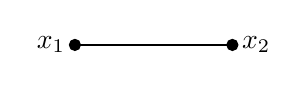
\begin{tikzpicture}[baseline={([yshift=-.5ex]current bounding box.center)}]
      \draw[thick] (0,0) -- (2,0);
      \filldraw[black] (0,0) circle (2pt) node[anchor=east]{\(x_1\)};
      \filldraw[black] (2,0) circle (2pt) node[anchor=west]{\(x_2\)};
    \end{tikzpicture}
  \end{align*}
  \caption{1 Way to Connect 2 points pairwise}
  \label{fig:n2}
\end{figure}
Hence we get our factor of $1!!=1$, and our single power of $a$. We could back this up further by considering the $n=0$ case, where we would only get a weight of 1, and no factors of $a^{-1}$, so we can interpret this as only 1 way to connect 0 points together with no lines.

The next case we did involved 4 points:
\begin{figure}[H]
  \centering
  \begin{align*}
    \ev{x^4}=
    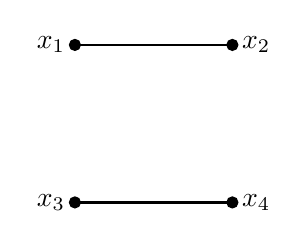
\begin{tikzpicture}[baseline=.9cm]
      \draw[thick] (0,0) -- (2,0);
      \draw[thick] (0,2) -- (2,2);
      \filldraw[black] (0,2) circle (2pt) node[anchor=east]{\(x_1\)};
      \filldraw[black] (2,2) circle (2pt) node[anchor=west]{\(x_2\)};
      \filldraw[black] (0,0) circle (2pt) node[anchor=east]{\(x_3\)};
      \filldraw[black] (2,0) circle (2pt) node[anchor=west]{\(x_4\)};
    \end{tikzpicture}+
    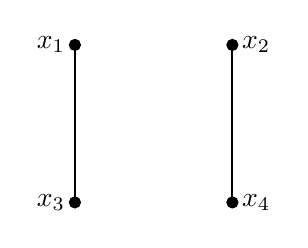
\begin{tikzpicture}[baseline=.9cm]
      \draw[thick] (0,0) -- (0,2);
      \draw[thick] (2,0) -- (2,2);
      \filldraw[black] (0,2) circle (2pt) node[anchor=east]{\(x_1\)};
      \filldraw[black] (2,2) circle (2pt) node[anchor=west]{\(x_2\)};
      \filldraw[black] (0,0) circle (2pt) node[anchor=east]{\(x_3\)};
      \filldraw[black] (2,0) circle (2pt) node[anchor=west]{\(x_4\)};
    \end{tikzpicture}+
    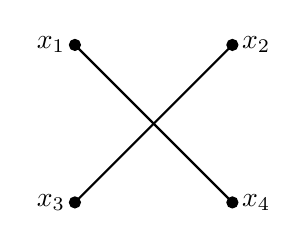
\begin{tikzpicture}[baseline=.9cm]
      \draw[thick] (0,0) -- (2,2);
      \draw[thick] (2,0) -- (0,2);
      \filldraw[black] (0,2) circle (2pt) node[anchor=east]{\(x_1\)};
      \filldraw[black] (2,2) circle (2pt) node[anchor=west]{\(x_2\)};
      \filldraw[black] (0,0) circle (2pt) node[anchor=east]{\(x_3\)};
      \filldraw[black] (2,0) circle (2pt) node[anchor=west]{\(x_4\)};
    \end{tikzpicture}
  \end{align*}
  \caption{3 Ways to Connect 2 points pairwise}
  \label{fig:n4}
\end{figure}
This gives our factor of $3!!=3$, and each only has two connections, so two powers of $a^{-1}$. 

One more constraint we have is that only even powers of $n$, so we have the following diagrammatic rules:
\begin{itemize}
\item Must connect $n$ points together pairwise
\item No points can be disconnected
\item A point cannot be connected to itself
\item $\ev{x^n}$ is the total number of diagrams divided $a$ to the number of lines used in each.
\end{itemize}

\subsection{Higher Dimensional Equivalent Integral}
In order to complete the square, we need to rewrite the argument of the exponential:
\begin{align*}
  -\frac12\vb{x}^T\vb{Ax}+\vb{b}^T\vb{x}=-\frac12\qty(\vb{x}^T\vb{Ax}-2\vb{b}^T\vb{x})
\end{align*}
We can then work only with the parenthetical quantity:
\begin{align*}
  \vb{x}^T\A\vb{x}-2\vb{b}^T\vb{x}
  &=\vb{x}^T\vb{Ax}-2\vb{b}^T\vb{x}+\vb{b}^T\A^{-1}\vb{b}-\vb{b}^T\A^{-1}\vb{b}\\
  &=\vb{x}^T\vb{Ax}-2\vb{b}^T\A^{-1}\A\vb{x}+
  \vb{b}^T\A^{-1}\A\A^{-1}\vb{b}-\vb{b}^T\A^{-1}\vb{b}\\
  &=(\vb{x}-\A^{-1}\vb{b})^T\A\vb{x}
  -\vb{b}^T\A^{-1}(\A\vb{x}-\A\A^{-1}\vb{b})-\vb{b}^T\A^{-1}\vb{b}\\
  &=(\vb{x}-\A^{-1}\vb{b})^T\A(\vb{x}-\A^{-1}\vb{b})-\vb{b}^T\A^{-1}\vb{b}
\end{align*}
We have used the fact that $\A$ (as well as its inverse) is symmetric. This gives our integrand:
\begin{align*}
  \exp{-\frac12(\vb{x}-\A^{-1}\vb{b})^T\A(\vb{x}-\A^{-1}\vb{b})+\frac12\vb{b}^T\A^{-1}\vb{b}}
  =e^{\frac12\vb{b}^T\A^{-1}\vb{b}}
  e^{-\frac12(\vb{x}-\A^{-1}\vb{b})^T\A(\vb{x}-\A^{-1}\vb{b})}
\end{align*}
We can separate the two terms as in the end they are scalars. The integral is then:
\begin{align*}
  \int\dd{x_1}\cdots\dd{x_N}e^{-\vb{x}^T\vb{Ax}/2+\vb{b}^T\vb{x}}
  =e^{\frac12\vb{b}^T\A^{-1}\vb{b}}\int\dd{x_1}\cdots\dd{x_N}
  e^{-\frac12(\vb{x}-\A^{-1}\vb{b})^T\A(\vb{x}-\A^{-1}\vb{b})}
\end{align*}
One simplification we can do now is shifting $\vb{x}$ to simplify the argument of the exponential, if we set:
\begin{align*}
  y_i=x_i-A_{ik}b_k
\end{align*}
However, there is no cause to be concerned, as if we compute the Jacobian, we find:
\begin{align*}
  J_{ij}=\pdv{y_i}{x_j}=\delta_{ij}
\end{align*}
Since $\A,\vb{b}$ are not dependent on $\vb{x}$, this means the determinant of the Jacobian will be $1$, such that
\begin{align*}
  e^{\frac12\vb{b}^T\A^{-1}\vb{b}}\int\dd{x_1}\cdots\dd{x_N}
  e^{-\frac12(\vb{x}-\A^{-1}\vb{b})^T\A(\vb{x}-\A^{-1}\vb{b})}
  =e^{\frac12\vb{b}^T\A^{-1}\vb{b}}\int\dd{y_1}\cdots\dd{y_N}
  e^{-\frac12\vb{y}^T\A\vb{y}}
\end{align*}
We should then derive the form of this integral:
\begin{align*}
  \int\dd{y_1}\cdots\dd{y_N}e^{-\frac12\vb{y}^T\A\vb{y}}
\end{align*}
We know that $\A$ is positive definite, so it is not only invertible, but diagonalizable, so there is a way to write $\A$ as:
\begin{align*}
  \A=\vb{P}^{-1}\vb{DP}
\end{align*}
Where $\vb{D}$ is a diagonal matrix with the eigenvalues of $\A$, $\lambda_i$ as its entries, and $P$ is orthogonal $P^T=P^{-1}$. We can then write the integral as:
\begin{align*}
  \int\dd{y_1}\cdots\dd{y_N}e^{-\frac12\vb{y}^T\A\vb{y}}=
  \int\dd{y_1}\cdots\dd{y_N}e^{-\frac12\vb{y}^T\vb{P}^T\vb{DP}\vb{y}}
  =\int\dd{y_1}\cdots\dd{y_N}e^{-\frac12(\vb{Py})^T\vb{D}(\vb{Py})}
\end{align*}
With another change of variables:
\begin{align*}
  \vb{z}=\vb{Py}\implies z_i=P_{ij}y_i\implies J_{ij}=\pdv{z_i}{y_j}=P_{ij}
\end{align*}
However, the determinant of $\vb{P}$ must be $1$ to keep the determinant of $A$ the same, so this actually does not change the integral:
\begin{align*}
  \int\dd{y_1}\cdots\dd{y_N}e^{-\frac12(\vb{Py})^T\vb{D}(\vb{Py})}
  =\int\dd{z_1}\cdots\dd{z_N}e^{-\frac12(\vb{z})^T\vb{D}(\vb{z})}
  =\int\dd{z_1}\cdots\dd{z_N}e^{-\frac12\lambda_iz_i^2}
\end{align*}
Where $i$ is summed over, so we have $N$ decoupled gaussians, one of which is given by:
\begin{align*}
  \int\dd{z_k}e^{-\frac12\lambda_kz_k^2}=\sqrt{\frac{2\pi}{\lambda_k}}
\end{align*}
Hence for all of the integrals we have:
\begin{align*}
  \int\dd{z_1}\cdots\dd{z_N}e^{-\frac12\lambda_iz_i^2}
  =\qty(2\pi)^{N/2}\qty(\prod_{i=1}^N\lambda_i)^{-1}
\end{align*}
The product of eigenvalues is also the determinant, and one over the determinant is the same as the determinant of the inverse, hence:
\begin{align*}
  \qty(2\pi)^{N/2}\qty(\prod_{i=1}^N\lambda_i)^{-1}=(2\pi)^{N/2}\qty(\det(\A))^{-1/2}
  =(2\pi)^{N/2}\sqrt{\det(\A^{-1})}
\end{align*}
So the original integral is:
\begin{align*}
  e^{\frac12\vb{b}^T\A^{-1}\vb{b}}\int\dd{x_1}\cdots\dd{x_N}e^{-\frac12\vb{y}^T\A\vb{y}}
  =e^{\frac12\vb{b}^T\A^{-1}\vb{b}}(2\pi)^{N/2}\sqrt{\det(\A^{-1})}
\end{align*}
Hence the result is:
\begin{align}
  \boxed{\int\dd{x_1}\cdots\dd{x_N}e^{-\vb{x}^T\vb{Ax}/2+\vb{b}^T\vb{x}}
    =e^{\frac12\vb{b}^T\A^{-1}\vb{b}}(2\pi)^{N/2}\sqrt{\det(\A^{-1})}}
\end{align}
All that is left is to is calculate $\ev{x_ix_j}$ and $\ev{x_ix_jx_kx_\ell}$.

First we have the integral in the denominator, which is given as the above result with $\vb{b}=\vb{0}$:
\begin{align*}
  \int\dd{x_1}\cdots\dd{x_N}e^{-\vb{x}^T\vb{Ax}/2}
  =(2\pi)^{N/2}\sqrt{\det(\A^{-1})}\equiv N(0)
\end{align*}
Where $N$ is given in general by:
\begin{align*}
  N(\vb{b})=\int\dd{x_1}\cdots\dd{x_N}e^{-\vb{x}^T\vb{Ax}/2+\vb{b}^T\vb{x}}
\end{align*}
Note that we have:
\begin{align*}
  \frac{N(\vb{b})}{N(0)}
  =e^{\frac12\vb{b}^T\A^{-1}\vb{b}}
\end{align*}
We can now see that this is the generating functions of the moments, with the $n=2$ moment being given by:
\begin{align*}
  \ev{x_ix_j}&=
  \eval{\pdv{b_i}\pdv{b_j}\qty(\exp{\frac12\vb{b}^T\A^{-1}\vb{b}})}_{\vb{b}=\vb{0}}\\
  &=\eval{\pdv{b_i}\pdv{b_j}\qty(\exp{\frac12b_i(\A^{-1})_{ij}b_j})}_{b_i=0}
\end{align*}
We will only need a few actual derivatives, listed here:
\begin{align*}
  \pdv{b_{i}}{b_k}&=\delta_{ik}\implies \pdv{C_{ij}b_j}{b_k}=C_{ij}\delta_{jk}=C_{ik}\\
  \pdv{b_{k}}\qty(b_iC_{ij}b_j)&=b_iC_{ik}+\underbrace{C_{kj}b_j}_{\text{symm.}}=2b_{j}C_{ij}\\
  \pdv{b_{k}}e^{b_iC_{ij}b_j/2}&=\frac12\pdv{b_{k}}\qty(b_iC_{ij}b_j)e^{b_iC_{ij}b_j/2}
  =\boxed{b_jC_{jk}e^{b_iC_{ij}b_j/2}}\\
\end{align*}
Everything else can be found via product or chain rule. Start with the derivatives of $\ev{x_ix_j}$, where we will use $k_i$ instead of $i,j$:
\begin{align*}
  \pdv{b_{k_1}}e^{b_i(A^{-1})_{ij}b_j/2}&=b_j(A^{-1})_{jk_1}e^{b_i(A^{-1})_{ij}b_j/2}\\
  \pdv{b_{k_2}}\pdv{b_{k_1}}e^{b_i(A^{-1})_{ij}b_j/2}
  &=\pdv{b_{k_2}}\qty(b_j(A^{-1})_{jk_1}e^{b_i(A^{-1})_{ij}b_j/2})\\
  &=\D_{k_2}\qty(b_j(A^{-1})_{jk_1})e^{b_i(A^{-1})_{ij}b_j/2}
  +b_j(A^{-1})_{jk_1}\D_{k_2}\qty(e^{b_i(A^{-1})_{ij}b_j/2})\\
  &=\qty((A^{-1})_{k_1k_2}+b_{j}(A^{-1})_{jk_1}b_{i}(A^{-1})_{ik_1})e^{b_i(A^{-1})_{ij}b_j/2}
\end{align*}
Cutting off here and settings $b_i=0$ will give us $\ev{x_{k_1}x_{k_2}}$:
\begin{align}
  \boxed{\ev{x_{k_1}x_{k_2}}=(A^{-1})_{k_1k_2}}
\end{align}
Continuing the derivatives from before we set the $\vb{b}$ term to $\vb{0}$:
\begin{align*}
  \frac{\D^3e^{b_i(A^{-1})_{ij}b_j/2}}{\D b_{k_3}\D b_{k_2}\D b_{k_1}}
  =&\ \D_{k_3}\qty(\qty((A^{-1})_{k_1k_2}+b_{j}(A^{-1})_{jk_1}b_{i}(A^{-1})_{ik_1})e^{b_i(A^{-1})_{ij}b_j/2})\\
  =&\ \left[(A^{-1})_{k_1k_2}(A^{-1})_{k_3j}b_j+(A^{-1})_{k_3k_2}(A^{-1})_{k_1j}b_j+(A^{-1})_{k_1k_3}(A^{-1})_{k_2j}b_j\right.\\
  &\ \left.+(A^{-1})_{k_1j}b_j(A^{-1})_{k_2m}b_m(A^{-1})_{k_3n}b_n\right]e^{b_i((A^{-1})^{-1})_{ij}b_j/2}
\end{align*}
The derivative of the above term is of the form:
\begin{align*}
  \frac{\D e^{b_i(A^{-1})_{ij}b_j/2}}{\D b_{k_4}\D b_{k_3}\D b_{k_2}\D b_{k_1}}=
  [(A^{-1})_{k_1k_3}(A^{-1})_{k_2k_4}+(A^{-1})_{k_2k_3}(A^{-1})_{k_1k_4}
  \\+(A^{-1})_{k_1k_2}(A^{-1})_{k_3k_4}
  +\order{b}]e^{b_i(A^{-1})_{ij}b_j/2}
\end{align*}
Such that when we take the $b_i\to0$, we get:
\begin{align*}
  \ev{x_{k_2}x_{k_2}x_{k_3}x_{k_4}}
  &=(A^{-1})_{k_1k_3}(A^{-1})_{k_2k_4}
  +(A^{-1})_{k_2k_3}(A^{-1})_{k_1k_4}
  +(A^{-1})_{k_1k_2}(A^{-1})_{k_3k_4}\\
  &=\ev{x_{k_1}x_{k_3}}\ev{x_{k_2}x_{k_4}}
  +\ev{x_{k_2}x_{k_3}}\ev{x_{k_1}x_{k_4}}
  +\ev{x_{k_1}x_{k_2}}\ev{x_{k_3}x_{k_4}}
\end{align*}
So the 4-point function can be completely written as a product of 2-point functions!
\begin{align}
  \boxed{\ev{x_{i}x_{j}x_{k}x_{\ell}}
    =\ev{x_{i}x_{k}}\ev{x_{j}x_{\ell}}
    +\ev{x_{j}x_{k}}\ev{x_{i}x_{\ell}}
    +\ev{x_{i}x_{j}}\ev{x_{k}x_{\ell}}}
\end{align}
With the general case, we can use a bit of physicist's induction, noticing that we have $(n-1)!!$ terms, we should connect it to the problem of matching up pairs of points:
\begin{align*}
  \ev{x_{i_1}\cdots x_{i_n}}=\sum_{\text{parings}}\ev{x_{j_1}x_{j_2}}\cdots\ev{x_{j_{(N-1)}}x_{j_N}}
\end{align*}
Where the number of pairings is the factor $(n-1)!!$ we found earlier. Also using a bit more of physicists induction, we can see that both terms with an odd number of derivatives would all disappear when $b_i=0$, so we can conclude:
\begin{align*}
  \ev{x_{i_1}\cdots x_{i_{(2m+1)}}}=0
\end{align*}
Hence the general form for even $n$ is:
\begin{align}
  \boxed{\ev{x_{i_1}\cdots x_{i_n}}=\sum_{\text{parings}}\ev{x_{j_1}x_{j_2}}\cdots\ev*{x_{j_{(N-1)}}x_{j_N}}}
\end{align}
\newpage

%% Problem 3
\section{Hubbard-Stratonovich Transformation}
\begin{problem}
  Consider the $\phi^4$ theory
  \begin{equation}
    \label{eq:1}
    \L=\frac12(\D_\mu\phi)^2-\frac12m^2\phi^2-\frac{g}{4!}\phi^4
  \end{equation}
  Now shift the Lagrangian by adding a new field $\sigma$ via:
  \begin{align*}
    \L'=\L+\frac1{6g}\qty(\sigma-\frac{g}2\phi^2)^2
  \end{align*}
  By performing a functional integral over the field $\sigma$, show that the new term doesn't change the dynamics of the theory. Confirm this by finding the Euler-Lagrange equation for $\sigma$ and showing that it has no time derivatives. This means that it can only provide a constraint, and $\sigma$ can be eliminated, much like the time component of a massive vector field.

  Write down the Feynman rules for the new theory. Compute the invariant amplitude for $\phi+\phi\to\phi+\phi$ scattering to order g, and show that it agrees with the amplitude computed in the theory \eqref{eq:1}.

  (To complete the so-called \emph{Hubbard-Stratonovich transformation}, one integrates out the original $\phi$ field, to obtain a non-local theory in terms of $\sigma$.)
\end{problem}

\subsection{Showing dynamics are unchanged}

Let $\Delta \L = \frac{1}{6g} (\sigma - \frac{g}{2} \phi^2)^2$ be the addition to our Lagrangian density. First, we will show that the contribution from $\Delta \L$ does not affect the n-point functions, and thus the dynamics of the theory are unchanged. Recall that the n-point function is given by

\begin{align*}
  G^{(n)}(x_1,...,x_n)=(-i)^n \frac{1}{Z[0]}\frac{\delta^n}{\delta J(x_1)...\delta J(x_n)}Z[J]|_{J=0} 
\end{align*}
Where the path integral with an added source is given by $Z[J]$ and the path integral without this added source is given by $Z[0]$. Thus, if the path integral is multiplied by a constant, it cancels between $Z[J]$ and $Z[0]$, and the n-point function/dynamics are unchanged.

For arbitrary constant $C$, we must then show:
\begin{align*}
  \int\mathcal{D}\sigma\mathcal{D}\phi e^{i S[\sigma,\phi]}=
  C\int \mathcal{D} \phi e^{i S[\phi]}
\end{align*}
where the actions $S$ are given by:
\begin{align*}
  S[\phi] &= \int d^4 x \L \\
  S[\sigma,\phi] &= \int d^4 x \L'= S[\phi] + \int d^4 x \Delta \L
\end{align*}
If we set:
\begin{align*}
  \Delta S \equiv \int d^4 x \Delta \L
\end{align*}
We see that what we really want to show is that performing the path integral over $\sigma$ leaves us with the original path integral:
\begin{align*}
  \int \mathcal{D} \sigma  e^{i \Delta S } = C
\end{align*}

Let us perform this path integral. Using the definition of functional integration:
\begin{align*}
  \int\mathcal{D}\sigma  e^{i \Delta S }
  =\int e^{i \Delta S }\prod_{x_i}\dd{\sigma (x_i)}
\end{align*}
We'd like to do each $\sigma (x_i)$ integral separately. Note that
\begin{align*}
  \Delta S = \int d^4x f(\sigma(x))=\sum_{x_i} f(\sigma(x_i))
\end{align*}
So we have
\begin{align*}
  \int\mathcal{D}\sigma  e^{i \Delta S }=
  \prod_{x_i}\int e^{i\Delta f(\sigma(x_i))}\dd{\sigma (x_i)}
\end{align*}
We can then just do each integral separately. Plugging in $\Delta \L$ for $f(\sigma(x_i))$, we have
\begin{align*}
  \int e^{if(\sigma(x_i))}\dd{\sigma(x_i)}
  =\int e^{i (\sigma(x_i)-g\phi^2/2)^2/(6g)}\dd{\sigma (x_i)}
\end{align*}
To do this integral, we can perform a change of variables. Let
\begin{align*}
  \sigma=\frac{g}{2} \phi^2 + e^{i\pi/4}\sigma'
\end{align*}
So that $\dd{\sigma} = e^{i\pi /4} \dd{\sigma'}$. Then our integral becomes
\begin{align*}
  I(\sigma_i)&\equiv \int e^{i (\sigma (x_i)-g\phi^2/2)^2/(6g) }\dd{\sigma (x_i)}
  =e^{i\pi /4} \int \dd{\sigma'}e^{i(e^{i\pi/4 \sigma'})^2g}\\
  &=e^{i\pi /4} \int \dd{\sigma'}e^{-\frac{1}{6g}(\sigma')^2}
  =e^{i\pi /4} \sqrt{6g\pi}
\end{align*}

Our integral became an easily solvable Gaussian integral, which gives us a constant! Since our integral is constant, the path integral over $\sigma$ is also constant:

\begin{align*}
  \int \mathcal{D} \sigma  e^{i \Delta S }=\prod_{x_i} I(\sigma_i)
\end{align*}
Hence we have shown reformulating the theory $\L$ as $\L'$ does not change the dynamics!

The Euler-Lagrange equations confirm this. Since the there are no $\Box \sigma$ or $\partial_\mu \sigma$ terms in the Lagrangian, applying the ELE equation for field $\sigma$ gives

\begin{align*}
  \pdv{\L}{\sigma}&=0 \implies 0=\frac{1}{3 g} \sigma-\frac{1}{6} \phi ^2
\end{align*}

Thus, $\sigma$ can be eliminated by setting
\begin{align}
  \boxed{\sigma=\frac{g}{2} \phi^2}
\end{align}
and is thus non-dynamical. 

\subsection{Feynman rules}
Now we compute the Feynman rules for each vertex we have in the new theory. Naiively, we will have a $\phi^4$ and a $\phi^2 \sigma$ vertex, since the squared terms just give propagators. However, note that the $\phi^4$ coefficients in $\L'$ cancel, so that we have no contribution from the $\phi^4$ vertex (or rather, we have a $\phi^4$ vertex with rule 0). Using solid lines for $\phi$ and dotted lines for $\sigma$, we have a vertex of this form
\begin{figure}[H]
  \centering
  \begin{tikzpicture}
    \begin{feynhand}
      \vertex (a) at (0,0);
      \vertex (c1) at (-1,-1) {$\phi$};
      \vertex (c2) at (-1, 1) {$\phi$};
      \vertex (b) at (1.5,0)  {$\sigma$};
      \propag (a) to (c1);
      \propag (a) to (c2);
      \propag[sca] (a) to (b);
    \end{feynhand}     
  \end{tikzpicture}
  \caption{Vertices for $\L'$ theory}
  \label{fig:vertices}
\end{figure}
Looking at the coefficients for this vertex term in the Lagrangian and noting the combinatoric factor of 2, we get the vertex rule:

\begin{align*}
  \begin{tikzpicture}[baseline=-2pt]
    \begin{feynhand}
      \vertex (a) at (0,0);
      \vertex (c1) at (-1,-1) {$\phi$};
      \vertex (c2) at (-1, 1) {$\phi$};
      \vertex (b) at (1.5,0)  {$\sigma$};
      \propag (a) to (c1);
      \propag (a) to (c2);
      \propag[sca] (a) to (b);
    \end{feynhand}     
  \end{tikzpicture}
  =\ \frac{i}{3}
\end{align*}

We also have propagators for $\sigma$ and $\phi$ particles:
\begin{figure}[H]
  \centering
  \begin{tikzpicture}
    \begin{feynhand}
      \vertex (a) at (0,0);
      \vertex (b) at (2,0);
      \propag[sca] (a) to [edge label=\(\sigma\)] (b);
    \end{feynhand}     
  \end{tikzpicture}
  \begin{tikzpicture}
    \begin{feynhand}
      \vertex (a) at (0,0);
      \vertex (b) at (2,0);
      \propag (a) to [edge label=\(\phi\)] (b);
    \end{feynhand}
  \end{tikzpicture}
  \caption{Propagators for $\L'$ theory}
  \label{fig:propagators}
\end{figure}

We have previously found the propagator for $\phi$:
\begin{align*}
  \begin{tikzpicture}[baseline=-2.7pt]
    \begin{feynhand}
      \vertex (a) at (0,0);
      \vertex (b) at (2,0);
      \propag (a) to [edge label=\(\phi\)] (b);
    \end{feynhand}
  \end{tikzpicture}
  =\frac{1}{(q^2-m^2)}
\end{align*}
The propagator for $\sigma$ can be found by noting that the Klein-Gordon equation for $\sigma$, since it is non-dynamical, reads:

\begin{align*}
  m^2 \sigma = J(x)
\end{align*}
So the Feynman propagator is given by the Green's function $D_F$ that satisfies
\begin{align*}
  m^2 D_F = -\delta (t'-t) \delta^{(3)} (\bf{x}'-\bf{x})
\end{align*}
Taking the Fourier transform to get the momentum space representation gives
\begin{align*}
  D_F = -\frac{1}{m_\sigma^2}=\frac{1}{1/(3g)}
\end{align*}
Where we have noted that the coefficient on $\sigma^2$ in $\L'$ gives $-m_{\sigma}^2=\frac{1}{3g}$.

Thus we have the rule:
\begin{align*}
  \begin{tikzpicture}[baseline=-2.7pt]
    \begin{feynhand}
      \vertex (a) at (0,0);
      \vertex (b) at (2,0);
      \propag [sca] (a) to [edge label=\(\sigma\)] (b);
    \end{feynhand}
  \end{tikzpicture}
  =i3g
\end{align*}

\subsection{Computing invariant amplitude}

Now we want to compute the invariant amplitude for $\phi + \phi \rightarrow \phi + \phi$ scattering at tree level. In our new theory, this is achieved through two vertices:

\begin{figure}[H]
  \centering
  \begin{tikzpicture}
    \begin{feynhand}
      \vertex (a) at (0,0);
      \vertex (c1) at (-1,-1) {$\phi$};
      \vertex (c2) at (-1, 1) {$\phi$};
      \vertex (b) at (1.5,0)  ;
      \vertex (d1) at (2.5,-1) {$\phi$};
      \vertex (d2) at (2.5,1) {$\phi$};
      \propag (a) to (c1);
      \propag (a) to (c2);
      \propag[sca] (a) to (b);
      \propag (b) to (d1);
      \propag (b) to (d2);
    \end{feynhand}     
  \end{tikzpicture}
  \\
  \begin{tikzpicture}
    \begin{feynhand}
      % vertices
      \vertex (p11) at (1.5,0) {$\phi$}; \vertex (p21) at (1.5,1.5) {$\phi$};
      \vertex (p12) at (-1.5,0) {$\phi$}; \vertex (p22) at (-1.5,1.5) {$\phi$};
      \vertex (a) at (0,0); \vertex (b) at (0,1.5);
      % particles
      \propag (p11) to (a); \propag (p12) to (a);
      \propag (b) to (p21); \propag (b) to (p22);
      \propag [sca] (a) to (b);
    \end{feynhand}
  \end{tikzpicture}
  \begin{tikzpicture}
    \begin{feynhand}
      % vertices
      \vertex (p11) at (1.5,0) {$\phi$}; \vertex (p21) at (1.5,1.5) {$\phi$};
      \vertex (p12) at (-1.5,0) {$\phi$}; \vertex (p22) at (-1.5,1.5) {$\phi$};
      \vertex (a) at (0,0); \vertex (b) at (0,1.5);
      % particles
      \propag (p21) to (a);
      \propag (p12) to (a);
      \propag (b) to (p11);
      \propag (b) to (p22);
      \propag [sca] (a) to (b);
    \end{feynhand}
  \end{tikzpicture}
  \caption{ $s$, $t$, and $u$ channel diagrams for $\phi + \phi\to \phi + \phi$ scattering in $\L'$ theory}
  \label{phiphiscattering}
\end{figure}

Note that since the propagator for $\sigma$ does not depend on momentum, each channel gives the same result and we can simply compute one channel's matrix element and multiply by 3. We have

\begin{align*}
  (2\pi)^4 \delta^4(p_1+p_2-p_3-p_4) \qty(- i \mathcal{M})&=3\qty(\frac{i}{3})^2\int \frac{\dd[4]{q}}{(2\pi)^4}
  \frac{i}{1/(3g)}\\&\times(2\pi)^4\delta ^4 (p_1+p_2-q) (2\pi )^4 \delta ^4 (q-p_3-p_4) \\
  -i\mathcal{M} &= -3 i\qty(\frac{1}{9}) \frac{1}{1/{(3g)}} = -i g
\end{align*}
Hence we arrive at the result
\begin{align}
  \implies \boxed{i\mathcal{M}= -i g}
\end{align}

In traditional $\phi^4$ theory, $\phi + \phi \rightarrow \phi + \phi$ scattering is done at tree level with only one vertex:
\begin{figure}[H]
  \centering
  \begin{tikzpicture}
    \begin{feynhand}
      % vertices
      \vertex (p11) at (-1,1) {$\phi$};
      \vertex (p12) at (-1,-1) {$\phi$};
      \vertex (p21) at (1,1) {$\phi$};
      \vertex (p22) at (1,-1) {$\phi$};
      \vertex (a) at (0,0);
      % particles
      \propag (p11) to (a);
      \propag (p12) to (a);
      \propag (a) to (p21);
      \propag (a) to (p22);
    \end{feynhand}
  \end{tikzpicture}
  \caption{$\phi + \phi\to \phi + \phi$ scattering in $\L$ theory}
  \label{fig:my_label}
\end{figure}
This vertex has rule 
\begin{align*}
  -i\mathcal{M} = -ig
\end{align*}
Which represents the entirety of the scattering process at tree level or order $g$. Thus, our invariant amplitudes for $\phi + \phi \rightarrow \phi +\phi$ scattering are the same regardless of using $\L$ or $\L ' $ theory.


\end{document}